\documentclass[10pt,aspectratio=169,t]{beamer}
\usepackage[T1]{fontenc}
\usepackage[scaled=0.94]{helvet}
\renewcommand{\familydefault}{\sfdefault}
\usepackage{amsmath,array,booktabs,graphicx,tabularx,tikz,xcolor,hyperref}
\usetikzlibrary{arrows.meta,positioning}

\definecolor{TTURed}{HTML}{CC0000}
\definecolor{CMSBlue}{HTML}{1F77B4}
\definecolor{CMSGreen}{HTML}{2CA02C}
\definecolor{CMSPurple}{HTML}{9467BD}
\definecolor{CMSGray}{HTML}{6B7280}
\definecolor{DarkInk}{HTML}{111111}
\hypersetup{colorlinks=true,urlcolor=CMSBlue,linkcolor=DarkInk}
\setbeamertemplate{navigation symbols}{}
\setbeamercolor{normal text}{fg=DarkInk,bg=white}
\setbeamercolor{frametitle}{fg=black,bg=white}
\setbeamercolor{structure}{fg=TTURed}
\setbeamerfont{frametitle}{size=\fontsize{21}{23},series=\bfseries}
\setbeamerfont{normal text}{size=\fontsize{14}{17}}
\setbeamersize{text margin left=0.52cm,text margin right=0.52cm}

\setbeamertemplate{headline}{%
  \leavevmode
  \begin{beamercolorbox}[wd=\paperwidth,ht=0.26cm,dp=0.02cm,rightskip=0.28cm]{structure}
    \hfill\includegraphics[height=0.20cm]{assets/ttu_wordmark_white.png}
  \end{beamercolorbox}
  \begin{beamercolorbox}[wd=\paperwidth,ht=0.055cm,dp=0cm]{structure}\end{beamercolorbox}
}
\setbeamertemplate{frametitle}{\vspace{0.11cm}\insertframetitle\par\vspace{0.04cm}}
\setbeamertemplate{footline}{%
  \begin{beamercolorbox}[wd=\paperwidth,ht=0.045cm,dp=0cm,leftskip=0.33cm,rightskip=0.33cm]{normal text}
    {\color{TTURed}\rule{0.94\paperwidth}{0.045cm}}
  \end{beamercolorbox}
  \hbox{
    \begin{beamercolorbox}[wd=.27\paperwidth,ht=2.2ex,dp=.75ex,leftskip=.38cm]{normal text}
      \fontsize{6.2}{7.0}\selectfont 20 Oct. 2026
    \end{beamercolorbox}
    \begin{beamercolorbox}[wd=.54\paperwidth,ht=2.2ex,dp=.75ex,center]{normal text}
      \fontsize{6.2}{7.0}\selectfont Chris Madrid, CPAD 2026
    \end{beamercolorbox}
    \begin{beamercolorbox}[wd=.19\paperwidth,ht=2.2ex,dp=.75ex,rightskip=.38cm plus1fil]{normal text}
      \hfill\fontsize{6.2}{7.0}\selectfont\insertframenumber
    \end{beamercolorbox}
  }
}
\newcommand{\source}[1]{%
  \begin{tikzpicture}[remember picture,overlay]
    \node[anchor=south west,text width=0.91\paperwidth,align=left]
      at ([xshift=0.52cm,yshift=0.56cm]current page.south west)
      {\fontsize{5.3}{6.0}\selectfont\color{CMSGray}#1};
  \end{tikzpicture}
}
\newcommand{\red}[1]{\textcolor{TTURed}{\bfseries #1}}
\newcommand{\blue}[1]{\textcolor{CMSBlue}{\bfseries #1}}
\newcommand{\green}[1]{\textcolor{CMSGreen}{\bfseries #1}}
\newcommand{\purple}[1]{\textcolor{CMSPurple}{\bfseries #1}}
\newcommand{\tightitem}{\setlength\itemsep{0.32em}\setlength\parskip{0pt}}
\newcolumntype{Y}{>{\raggedright\arraybackslash}X}

\title{FLASH digital SiPM readout for fiber calorimetry}
\author{Chris Madrid}
\institute{Texas Tech University and the SLAC LDRD collaboration}
\date{CPAD 2026, Seattle}
\begin{document}

% 1
\begin{frame}[plain]
  \vspace{0.70cm}
  {\fontsize{27}{31}\selectfont\bfseries
    FLASH digital SiPM readout\par
    for time-resolved fiber calorimetry\par}
  \vspace{0.26cm}
  {\fontsize{14.5}{17}\selectfont
    From the CPAD 2025 sensor study to full-detector requirements\par}
  \vspace{0.20cm}
  {\fontsize{11.5}{14}\selectfont\color{TTURed}\bfseries
    SLAC Laboratory Directed Research and Development program\par}
  \vfill
  \begin{columns}[b,onlytextwidth]
    \begin{column}{0.18\textwidth}
      \includegraphics[height=1.38cm]{assets/particle_detector_lab.jpeg}
    \end{column}
    \begin{column}{0.80\textwidth}
      {\fontsize{14}{17}\selectfont\bfseries Chris Madrid\par}
      {\fontsize{10.5}{13}\selectfont Texas Tech University\par}
      {\fontsize{10.5}{13}\selectfont CPAD 2026, Seattle, 20 October 2026\par}
    \end{column}
  \end{columns}
  \vspace{0.24cm}
\end{frame}

% 2
\begin{frame}{CPAD 2025 established the starting point}
  \vspace{0.06cm}
  \begin{columns}[T,onlytextwidth]
    \begin{column}{0.47\textwidth}
      {\large\bfseries The 2025 study}\par
      \vspace{0.14cm}
      \begin{itemize}\tightitem
        \item introduced digital SiPM readout for HG-DREAM
        \item simulated photon occupancy in one Cherenkov fiber
        \item scanned SPAD size and 5--30 ns dead time
        \item reported a 25 $\mu$m scale and an initial timing/ML study
      \end{itemize}
    \end{column}
    \begin{column}{0.49\textwidth}
      {\large\bfseries The question left open}\par
      \vspace{0.18cm}
      \begin{center}
        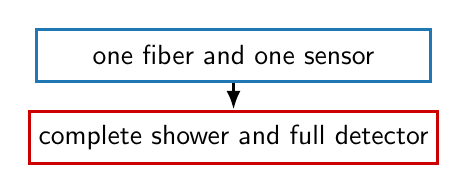
\begin{tikzpicture}[node distance=0.34cm]
          \node[draw=CMSBlue,line width=1.2pt,minimum width=5.0cm,minimum height=.66cm] (fiber) {one fiber and one sensor};
          \node[draw=TTURed,line width=1.2pt,minimum width=5.0cm,minimum height=.66cm,below=of fiber] (det) {complete shower and full detector};
          \draw[-{Latex[length=2.4mm]},line width=1.2pt] (fiber)--(det);
        \end{tikzpicture}
      \end{center}
      \vspace{0.12cm}
      \small Does a candidate dSiPM preserve the calorimeter response after
      calibration, recovery, and realistic shower occupancy?
    \end{column}
  \end{columns}
  \source{L. Wu et al., Study of Digital Silicon Photomultiplier Specifications for a High-Granularity Calorimeter with Simulations, CPAD 2025.}
\end{frame}

% 3
\begin{frame}{Progress since CPAD 2025}
  \fontsize{9.1}{10.9}\selectfont
  \begin{tabularx}{\textwidth}{>{\raggedright\arraybackslash\bfseries}p{3.0cm} Y Y}
    \toprule
    Topic & CPAD 2025 & CPAD 2026 status \\
    \midrule
    Program & concept and simulation study &
      funded SLAC LDRD for FLASH prototype development \\
    Software & one-fiber occupancy plots &
      exact historical reproduction, deterministic response model, 28 tests \\
    Geometry & displayed segmentation scale &
      physical millimeter coordinates and corrected pitch interpretation \\
    Sensor response & SPAD size and fixed dead time &
      joint PDE, pitch, recovery, event-tail, and pulse-shape studies \\
    Detector physics & local fiber response &
      full-detector Cherenkov mapping and calibrated response transfer \\
    Reference readout & qualitative analog comparison &
      conventional SiPM partial-recharge proxy on the same photons \\
    \bottomrule
  \end{tabularx}
  \vspace{0.22cm}
  \centering\red{The LDRD now has a validated simulation chain that can ingest prototype measurements.}
\end{frame}

% 4
\begin{frame}{HG-DREAM defines the detector benchmark}
  \begin{columns}[T,onlytextwidth]
    \begin{column}{0.55\textwidth}
      \includegraphics[width=\linewidth,height=0.58\textheight,keepaspectratio]{assets/hgdream_detector_photo.png}
    \end{column}
    \begin{column}{0.42\textwidth}
      \vspace{0.08cm}
      \begin{itemize}\tightitem
        \item dense Cherenkov and scintillation fiber readout
        \item bright electromagnetic shower cores
        \item fine transverse segmentation
        \item 2 m optical path with depth-dependent timing
        \item beam data and present analog waveform readout for closure
      \end{itemize}
      \vspace{0.24cm}
      \red{Core question}\par
      \small Can FLASH replace the photosensor/readout layer while preserving
      energy, imaging, and timing information?
    \end{column}
  \end{columns}
  \source{HG-DREAM image and detector description: Y. Feng, CALOR 2026; C. Madrid, Higgs 2025.}
\end{frame}

% 5
\begin{frame}{Analysis chain and validation gates}
  \fontsize{9.6}{11.4}\selectfont
  \begin{tabularx}{\textwidth}{>{\raggedright\arraybackslash\bfseries}p{2.8cm} Y Y}
    \toprule
    Stage & Calculation & Required check \\
    \midrule
    Optical input & Geant4 photon position, time, wavelength, fiber identity &
      cutflow, containment, event statistics \\
    Sensor response & PDE selection, physical cell mapping, recovery &
      deterministic seeds, exact limiting cases, historical closure \\
    Channel output & photon count, retained time profile, analog charge proxy &
      linear baseline at the same PDE \\
    Detector output & calibrated C response and illustrative dual-readout transfer &
      branch correlation, sample provenance, explicit scope limits \\
    \bottomrule
  \end{tabularx}
  \vspace{0.30cm}
  \begin{columns}[T,onlytextwidth]
    \begin{column}{0.49\textwidth}
      \blue{One-fiber samples}\par
      \small 5,000 events each, used as unmatched-energy occupancy stress tests.
    \end{column}
    \begin{column}{0.49\textwidth}
      \red{Full-detector samples}\par
      \small 1,000 positron and 100 pion events, used for response-transfer tests.
    \end{column}
  \end{columns}
\end{frame}

% 6
\begin{frame}{Fiber-face photon density: ensemble view}
  \centering
  \includegraphics[width=0.95\textwidth,height=0.67\textheight,keepaspectratio]{assets/photon_xy_comparison.pdf}
  \vspace{-0.03cm}
  \parbox{0.94\textwidth}{\centering\fontsize{8.6}{10.0}\selectfont
  Square axes preserve the 0.8 mm fiber geometry. The accumulated maps expose
  the edge enhancement that drives local SPAD occupancy.}
\end{frame}

% 6b
\begin{frame}{Fiber-face photon density: one event}
  \centering
  \includegraphics[width=0.92\textwidth,height=0.61\textheight,keepaspectratio]{assets/photon_xy_single_event.pdf}
  \vspace{-0.04cm}
  \parbox{0.94\textwidth}{\centering\fontsize{8.6}{10.0}\selectfont
  One objectively selected median-count event per sample. The sparse photon pattern---not
  the smooth ensemble average---is what FLASH digitizes.}
\end{frame}

% 7
\begin{frame}{Historical closure and physical pitch}
  \centering
  \includegraphics[width=0.86\textwidth,height=0.66\textheight,keepaspectratio]{assets/v2_mapping_correction.png}
  \vspace{-0.02cm}
  \parbox{0.94\textwidth}{\centering\fontsize{8.5}{9.9}\selectfont
  The 2025 histograms reproduce exactly. The old 3 mm segmentation was applied
  across a 1 mm DREAMSim display range, so the labeled pitch acted as
  \red{one third of the physical pitch}.}
  \source{Historical sequence: C. Madrid and S. McKinley, Digital SiPM Light Occupancy Study, 2025.}
\end{frame}

% 8
\begin{frame}{Physical segmentation and repeated hits}
  \centering
  \includegraphics[width=0.94\textwidth,height=0.66\textheight,keepaspectratio]{assets/one_fiber_segmentation.png}
  \vspace{-0.03cm}
  \parbox{0.94\textwidth}{\centering\fontsize{8.6}{10.0}\selectfont
  The reproduced multiplicity distributions now carry physical pitch labels.
  Finer cells suppress the multi-photon tail before recovery is applied.}
\end{frame}

% 9
\begin{frame}{PDE, pitch, and recovery operating surface}
  \centering
  \includegraphics[width=0.94\textwidth,height=0.66\textheight,keepaspectratio]{assets/v2_physical_requirements.png}
  \vspace{-0.03cm}
  \parbox{0.95\textwidth}{\centering\fontsize{8.6}{10.0}\selectfont
  In the 1 TeV pion stress sample, 20 $\mu$m pitch, 20\% PDE, and 4.3 ns
  recovery retains \red{92.7\%} of detected photons. No single pitch
  requirement survives changes in PDE, recovery, or photon density.}
\end{frame}

% 9a
\begin{frame}{Pitch is not the photosensitive area}
  \centering
  \includegraphics[width=0.95\textwidth,height=0.66\textheight,keepaspectratio]{assets/fill_factor_pitch_matrix.png}
  \vspace{-0.03cm}
  \parbox{0.95\textwidth}{\centering\fontsize{8.5}{9.9}\selectfont
  The response is now factorized into active area, wavelength-dependent
  junction detection, SPAD recovery, and shared-channel output. At 20 $\mu$m
  pitch and 70\% fill, the proxy gives 18.74\% effective detection, 93.06\%
  recovery survival, and 16.79 exported timestamps per 100 incident photons.}
  \source{Square active-area and capstone spectral-shape proxies; 30\% peak junction PDE. These are requirement assumptions, not FLASH measurements.}
\end{frame}

% 9b
\begin{frame}{Readout grouping creates a second dynamic range}
  \centering
  \includegraphics[width=0.91\textwidth,height=0.56\textheight,keepaspectratio]{assets/channel_architecture_matrix.png}
  \vspace{-0.10cm}
  \parbox{0.94\textwidth}{\centering\fontsize{8.0}{9.2}\selectfont
  An eight-word buffer selects a \red{50--100 $\mu$m} timing-channel scale
  across this pitch scan. Pitch, active junction, timing-group size, and output
  policy are separate requirements.}
  \source{1 TeV pion stress sample; 20\% PDE, 4.3 ns recovery, and 50 ps channel resolving time.}
\end{frame}

% 10
\begin{frame}{Recovery-driven pulse-shape distortion}
  \centering
  \includegraphics[width=0.84\textwidth,height=0.66\textheight,keepaspectratio]{assets/v2_pulse_shape.png}
  \vspace{-0.03cm}
  \parbox{0.93\textwidth}{\centering\fontsize{8.6}{10.0}\selectfont
  Repeated hits cluster near the prompt peak. Total photon retention can remain
  high while early-time fractions and leading-edge observables shift.}
\end{frame}

% 11
\begin{frame}{One-fiber result and its statistical boundary}
  \begin{columns}[T,onlytextwidth]
    \begin{column}{0.58\textwidth}
      \includegraphics[width=\linewidth,height=0.55\textheight,keepaspectratio]{assets/v2_event_tail.png}
    \end{column}
    \begin{column}{0.39\textwidth}
      \vspace{0.10cm}
      \small At 20\% PDE and 4.3 ns recovery in the pion stress sample:
      \vspace{0.14cm}
      \begin{tabular}{rcc}
        \toprule
        pitch & mean & 10th percentile \\
        \midrule
        10 $\mu$m & 97.9\% & 96.7\% \\
        20 $\mu$m & 92.7\% & 90.3\% \\
        25 $\mu$m & 89.5\% & 86.2\% \\
        \bottomrule
      \end{tabular}
      \vspace{0.24cm}

      Bright-event tails strengthen the requirement. The 100 GeV positron
      and 1 TeV pion files remain occupancy stress samples, not a controlled
      species comparison.
    \end{column}
  \end{columns}
\end{frame}

% 12
\begin{frame}{Full-detector sample and branch audit}
  \centering
  \includegraphics[width=0.92\textwidth,height=0.63\textheight,keepaspectratio]{assets/full_detector_validation.png}
  \vspace{-0.02cm}
  \parbox{0.94\textwidth}{\centering\fontsize{8.4}{9.8}\selectfont
  Explicit Cherenkov photons track the stored C signal with $r=0.73$ for
  positrons and $r=0.90$ for pions. The two observables remain separate
  throughout the response study.}
\end{frame}

% 13
\begin{frame}{FLASH approaches the information limit}
  \centering
  \includegraphics[width=0.99\textwidth,height=0.73\textheight,keepaspectratio]{assets/full_detector_event_display.pdf}
  \vspace{-0.02cm}
  \parbox{0.96\textwidth}{\centering\fontsize{8.0}{9.2}\selectfont
  Same 90 GeV pion and axes. Each panel uses an independent robust logarithmic
  range. Extreme bins are clipped. Color shows
  $100N_{\mathrm{shown}}/(N_{\mathrm{incident}}A_{\mathrm{channel}})$ in
  \% mm$^{-2}$. White means zero. Compare structure, not hue,
  across panels. Area normalization removes the HG-DREAM core/outer size bias.
  Ideal truth uses 2.0 mm display markers at the centers of physical 0.8 mm
  Cherenkov fibers. After 20\% PDE and 4.3 ns recovery, FLASH preserves much
  of that transverse structure.}
  \source{Geometry: N. Akchurin et al., NIM A 548 (2005) 336; S. Kunori, CALOR 2024; TTU FERS map, 2025 test beam.}
\end{frame}

% 14
\begin{frame}{Local dynamic range in complete showers}
  \centering
  \includegraphics[width=0.94\textwidth,height=0.61\textheight,keepaspectratio]{assets/full_detector_occupancy.png}
  \vspace{-0.03cm}
  \parbox{0.94\textwidth}{\centering\fontsize{8.4}{9.8}\selectfont
  The brightest-fiber median is 621 photons for 100 GeV positrons and 145 for
  90 GeV pions. The conventional proxy retains 88.5\%/96.9\% of
  positron/pion charge. FLASH retains 97.8\%/99.4\% of detected hits.}
\end{frame}

% 15
\begin{frame}{Particle-dependent Cherenkov response transfer}
  \centering
  \includegraphics[width=0.93\textwidth,height=0.60\textheight,keepaspectratio]{assets/full_detector_performance_scan.png}
  \vspace{-0.02cm}
  \parbox{0.95\textwidth}{\centering\fontsize{8.5}{9.9}\selectfont
  Electron calibration produces a \purple{$+9.5\%$} pion C shift for the
  representative C-Series proxy and a \blue{$+1.7\%$} shift for the
  20 $\mu$m, 4.3 ns FLASH point. Narrower response curves here reflect
  nonlinear compression.}
\end{frame}

% 16
\begin{frame}{Event-level response propagation}
  \centering
  \includegraphics[width=0.93\textwidth,height=0.61\textheight,keepaspectratio]{assets/full_detector_response.png}
  \vspace{-0.01cm}
  \parbox{0.94\textwidth}{\centering\fontsize{8.4}{9.8}\selectfont
  The left panel shows calibrated Cherenkov response. The right panel applies
  a fixed dual-readout coefficient as a sensitivity test. A final resolution
  result requires matched explicit C and S photon samples.}
\end{frame}

% 17
\begin{frame}{Longitudinal timing information in the current samples}
  \begin{columns}[T,onlytextwidth]
    \begin{column}{0.60\textwidth}
      \includegraphics[width=\linewidth,height=0.60\textheight,keepaspectratio]{assets/v2_timing_depth.png}
    \end{column}
    \begin{column}{0.37\textwidth}
      \vspace{0.06cm}
      \small A simple early-photon quantile predicts mean production depth with:
      \vspace{0.12cm}
      \begin{itemize}\tightitem
        \item 236 mm ideal-time RMSE
        \item 59 mm median absolute error
        \item less than 0.1 mm added RMSE for 50 ps response plus 50 ps TDC
        \item about 12 mm added RMSE for 1.145 ns response
      \end{itemize}
      \vspace{0.12cm}
      Shower and transport tails limit this proxy. Richer timing observables
      must set the 10--50 ps system requirement.
    \end{column}
  \end{columns}
\end{frame}

% 18
\begin{frame}{LDRD simulation progress and prototype inputs}
  \fontsize{9.0}{10.8}\selectfont
  \begin{tabularx}{\textwidth}{>{\raggedright\arraybackslash\bfseries}p{3.1cm} Y Y}
    \toprule
    Requirement & Simulation status & Prototype input \\
    \midrule
    Photon yield & deterministic PDE scan complete &
      PDE versus wavelength and overvoltage \\
    Local dynamic range & physical pitch and recovery surface complete &
      two-pulse recharge and bright-pulse response \\
    Timing response & arrival-time and depth baselines complete &
      sensor IRF, TDC binning, channel skew \\
    Noise and masking & software interfaces identified &
      DCR, crosstalk, afterpulsing, hot-cell maps \\
    Output policy & pitch/grouping scan with counters and finite buffers complete &
      timestamp mode, arbitration, measured record format \\
    Detector impact & first full-detector C response complete &
      measured analog chain and matched C/S production \\
    \bottomrule
  \end{tabularx}
  \vspace{0.22cm}
  \centering\red{Each bench measurement now updates a named simulation parameter and detector observable.}
\end{frame}

% 19
\begin{frame}{Next simulation and hardware milestones}
  \begin{columns}[T,onlytextwidth]
    \begin{column}{0.48\textwidth}
      {\large\bfseries Simulation production}\par
      \vspace{0.14cm}
      \begin{itemize}\tightitem
        \item matched $e$, $\pi$, and $\mu$ samples at 10, 30, 100, and 300 GeV
        \item at least 5,000 events per point
        \item explicit Cherenkov and scintillation photons
        \item present waveform and FLASH digitization on the same photons
      \end{itemize}
    \end{column}
    \begin{column}{0.48\textwidth}
      {\large\bfseries LDRD prototype closure}\par
      \vspace{0.14cm}
      \begin{itemize}\tightitem
        \item measured spectral PDE and timing response
        \item recovery under single- and double-pulse illumination
        \item realistic masking and correlated noise
        \item output modes evaluated against energy, imaging, and timing
      \end{itemize}
    \end{column}
  \end{columns}
  \vspace{0.28cm}
  \centering\red{Decision metric: detector performance versus active area, power, and event payload.}
\end{frame}

% 20
\begin{frame}{Conclusions}
  \vspace{0.10cm}
  \begin{itemize}\setlength\itemsep{0.48em}
    \item CPAD 2025 established the dSiPM occupancy problem for one HG-DREAM fiber.
    \item The 2026 audit reproduced that work and corrected the physical pitch interpretation.
    \item The updated study constrains PDE, pitch, recovery, event tails, and pulse shape together.
    \item Active-area fill factor and shared readout-channel size are now separated from physical pitch.
    \item Full-detector propagation shows a 1.7\% pion C shift for the selected FLASH point, compared with 9.5\% for a representative analog-SiPM proxy.
    \item The funded SLAC LDRD now has a validated simulation framework and a defined prototype measurement program.
  \end{itemize}
  \vfill
  \centering{\large\bfseries Next result: matched C/S photons and measured readout response in one detector-level comparison.}
\end{frame}

\appendix

% 21
\begin{frame}{Backup: CPAD 2025 claims under test}
  \fontsize{8.8}{10.6}\selectfont
  \begin{tabularx}{\textwidth}{>{\raggedright\arraybackslash\bfseries}p{4.2cm} Y >{\raggedright\arraybackslash}p{2.2cm}}
    \toprule
    2025 statement & 2026 finding & Status \\
    \midrule
    25 $\mu$m maximum SPAD size & original coordinate scale acted three times finer & superseded \\
    few-ns dead time has modest loss & true only on a PDE-pitch-density surface & refined \\
    one-fiber occupancy guides design & useful local stress test & retained \\
    timing may improve reconstruction & information exists, simple proxy remains shower limited & open \\
    dSiPM reduces readout burden & requires output-policy and bandwidth study & open \\
    \bottomrule
  \end{tabularx}
  \source{Baseline statements summarized from the public CPAD 2025 dSiPM talk.}
\end{frame}

% 22
\begin{frame}{Backup: full-detector input statistics}
  \small
  \begin{tabularx}{\textwidth}{>{\bfseries}l r r r r}
    \toprule
    Sample & events & C photons/event & active fibers/event & hottest fiber median \\
    \midrule
    100 GeV $e^+$ & 1000 & 13,749 & 841 & 621 \\
    90 GeV $\pi^+$ & 100 & 9,377 & 1,386 & 145 \\
    \bottomrule
  \end{tabularx}
  \vspace{0.30cm}
  \begin{itemize}\tightitem
    \item Selection uses valid Cherenkov fibers, positive sensor-plane exit, and a 0--40 ns gate.
    \item Four local fiber centers repeat on the 4 mm rod lattice.
    \item The 3 mm sensor contains all selected fiber-core endpoints.
  \end{itemize}
\end{frame}

% 23
\begin{frame}{Backup: historical software closure}
  \centering
  \includegraphics[width=0.91\textwidth,height=0.68\textheight,keepaspectratio]{assets/validation_historical_closure.png}
  \vspace{-0.03cm}
  \small Saved ROOT histograms, binning, and one-hit efficiency reproduce the historical calculation.
\end{frame}

% 24
\begin{frame}{Backup: repeated hits in one event}
  \centering
  \includegraphics[width=0.96\textwidth,height=0.68\textheight,keepaspectratio]{assets/validation_event_occupancy.png}
  \vspace{-0.03cm}
  \small The validation view exposes incident, detected, accepted, and lost photons cell by cell.
\end{frame}

% 25
\begin{frame}{Backup: conventional-SiPM proxy}
  \small
  \begin{tabularx}{\textwidth}{>{\raggedright\arraybackslash\bfseries}p{4.0cm} Y}
    \toprule
    Input & Representative Onsemi MicroFC-30035 value \\
    \midrule
    Active area & 3 $\times$ 3 mm$^2$ \\
    Peak PDE & 31\% at 420 nm and 2.5 V overvoltage \\
    Microcells & 4,774 data-sheet cells; 4,761-cell square model \\
    Recharge time constant & 82 ns \\
    Fast-output FWHM & 1.5 ns \\
    Charge model & $q=1-\exp(-\Delta t/82\,\mathrm{ns})$ for a repeated cell \\
    \bottomrule
  \end{tabularx}
  \vspace{0.22cm}
  The proxy excludes wavelength-dependent PDE, recharge-dependent trigger
  probability, crosstalk, afterpulsing, electronics noise, and waveform integration.
  \source{Onsemi, C-Series Silicon Photomultipliers, MicroC-SERIES data sheet, Rev. 7.}
\end{frame}

% 26
\begin{frame}{Backup: Cherenkov and scintillation scope}
  \centering
  \includegraphics[width=0.90\textwidth,height=0.61\textheight,keepaspectratio]{assets/full_detector_validation.png}
  \vspace{-0.02cm}
  \parbox{0.94\textwidth}{\centering\fontsize{8.6}{10.0}\selectfont
  The available full-detector files contain explicit Cherenkov photons and a
  stored scintillation sum. They do not contain an explicit scintillation
  photon population. The final dual-readout comparison therefore requires new
  matched production.}
\end{frame}

% 27
\begin{frame}{Backup: reproducibility record}
  \small The canonical rebuild performs these steps from local ROOT inputs:
  \begin{enumerate}\tightitem
    \item run 23 unit tests
    \item reproduce the 2025 electron and pion study
    \item rebuild audience and validation figures
    \item rerun the corrected one-fiber study with 500 bootstrap replicas
    \item rerun the full-detector digitization without cached event tables
    \item compile the deck and paper and record SHA-256 hashes
  \end{enumerate}
  \vspace{0.20cm}
  \texttt{results/cpad2026-rebuild/rebuild\_manifest.json} records the
  commands, input hashes, output hashes, and runtime.
\end{frame}

\end{document}
